\documentclass{extbook}[14pt]
\usepackage{multicol, enumerate, enumitem, hyperref, color, soul, setspace, parskip, fancyhdr, amssymb, amsthm, amsmath, latexsym, units, mathtools}
\everymath{\displaystyle}
\usepackage[headsep=0.5cm,headheight=0cm, left=1 in,right= 1 in,top= 1 in,bottom= 1 in]{geometry}
\usepackage{dashrule}  % Package to use the command below to create lines between items
\newcommand{\litem}[1]{\item #1

\rule{\textwidth}{0.4pt}}
\pagestyle{fancy}
\lhead{}
\chead{Answer Key for Progress Quiz 5 Version ALL}
\rhead{}
\lfoot{8497-6012}
\cfoot{}
\rfoot{Summer C 2021}
\begin{document}
\textbf{This key should allow you to understand why you choose the option you did (beyond just getting a question right or wrong). \href{https://xronos.clas.ufl.edu/mac1105spring2020/courseDescriptionAndMisc/Exams/LearningFromResults}{More instructions on how to use this key can be found here}.}

\textbf{If you have a suggestion to make the keys better, \href{https://forms.gle/CZkbZmPbC9XALEE88}{please fill out the short survey here}.}

\textit{Note: This key is auto-generated and may contain issues and/or errors. The keys are reviewed after each exam to ensure grading is done accurately. If there are issues (like duplicate options), they are noted in the offline gradebook. The keys are a work-in-progress to give students as many resources to improve as possible.}

\rule{\textwidth}{0.4pt}

\begin{enumerate}\litem{
For the scenario below, use the model for the volume of a cylinder as $V = \pi r^2 h$.

\begin{center}
    \textit{ Pringles wants to add 23 \text{percent} more chips to their cylinder cans and minimize the design change of their cans. They've decided that the best way to minimize the design change is to increase the radius and height by the same percentage. What should this increase be? }
\end{center}
The solution is \( \text{About } 7 \text{ percent} \), which is option D.\begin{enumerate}[label=\Alph*.]
\item \( \text{About } 11 \text{ percent} \)

This corresponds to solving correctly but treating both radius and height as equal contributors to the volume.
\item \( \text{About } 3 \text{ percent} \)

This corresponds to not solving for the increase properly.
\item \( \text{About } 12 \text{ percent} \)

This corresponds to treating both radius and height as equal contributors and not solving correctly.
\item \( \text{About } 7 \text{ percent} \)

* This is the correct option.
\item \( \text{None of the above} \)

If you chose this, please contact the coordinator to discus how you solved the problem.
\end{enumerate}

\textbf{General Comment:} Remember that when plugging the increases of values in, you need to treat it as that percentage above 100. For example, a 5 percent increase means 105 percent.
}
\litem{
Solve the modeling problem below, if possible.

\begin{center}
    \textit{ In CHM2045L, Brittany created a 18 liter 10 percent solution of chemical $\chi$ using two different solution percentages of chemical $\chi$. When she went to write her lab report, she realized she forgot to write the amount of each solution she used! If she remembers she used 5 percent and 28 percent solutions, what was the amount she used of the 5 percent solution? }
\end{center}
The solution is \( 14.09 liters \), which is option D.\begin{enumerate}[label=\Alph*.]
\item \( 3.91 liters \)

This is the concentration of 28 percent solution.
\item \( 9.00 liters \)

This would be correct if Brittany used equal parts of each solution.
\item \( 9.48 liters \)

This was a random value. If this was not a guess, contact the coordinator to talk about how you got this value.
\item \( 14.09 liters \)

*This is the correct option.
\item \( \text{There is not enough information to solve the problem.} \)

You may have chose this if you thought you needed to know how much of the second solution was used in the problem. Remember that the total minus the first solution would give you the second amount used.
\end{enumerate}

\textbf{General Comment:} Build the model exactly as you did in Module 9M. Then, solve for the volume you are looking for.
}
\litem{
Solve the modeling problem below, if possible.

\begin{center}
    \textit{ A new virus is spreading throughout the world. There were initially 8 many cases reported, but the number of confirmed cases has doubled every 5 days. How long will it be until there are at least 1000000 confirmed cases? }
\end{center}
The solution is \( \text{About } 85 \text{ days} \), which is option B.\begin{enumerate}[label=\Alph*.]
\item \( \text{About } 25 \text{ days} \)

You modeled the situation correctly but did not apply the properties of log correctly.
\item \( \text{About } 85 \text{ days} \)

* This is the correct option.
\item \( \text{About } 23 \text{ days} \)

You modeled the situation with $e$ as the base and did not apply the properties of log correctly.
\item \( \text{About } 59 \text{ days} \)

You modeled the situation with $e$ as the base, but solved correctly otherwise.
\item \( \text{There is not enough information to solve the problem.} \)

If you chose this option, please contact the coordinator to discuss why you think this is the case.
\end{enumerate}

\textbf{General Comment:} Set up the model the same as in Module 11M. Then, plug in 1000000 and solve for $d$ in your model.
}
\litem{
Determine the appropriate model for the graph of points below.

\begin{center}
    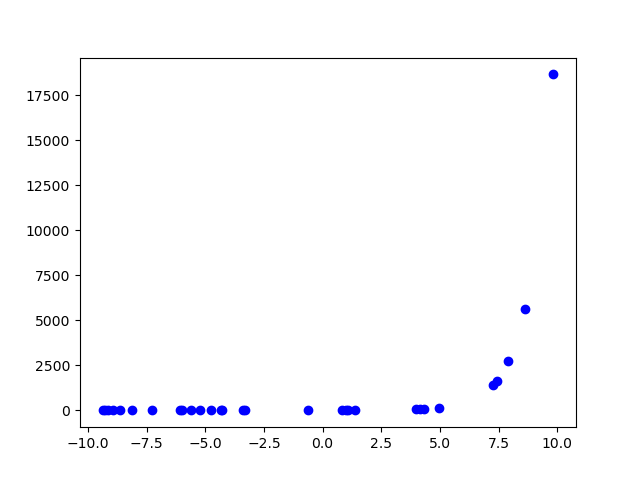
\includegraphics[width=0.5\textwidth]{../Figures/identifyModelGraph12A.png}
\end{center}


The solution is \( \text{Exponential model} \), which is option B.\begin{enumerate}[label=\Alph*.]
\item \( \text{Logarithmic model} \)

For this to be the correct option, we want a rapid change early, then an extremely slow change later.
\item \( \text{Exponential model} \)

For this to be the correct option, we want an extremely slow change early, then a rapid change later.
\item \( \text{Non-linear Power model} \)

For this to be the correct option, we need to see a polynomial or rational shape.
\item \( \text{Linear model} \)

For this to be the correct option, we need to see a mostly straight line of points.
\item \( \text{None of the above} \)

For this to be the correct option, we want to see no pattern in the points.
\end{enumerate}

\textbf{General Comment:} This question is testing if you can associate the models with their graphical representation. If you are having trouble, go back to the corresponding Core module to learn about the specific function you are having trouble recognizing.
}
\litem{
For the information provided below, construct a linear model that describes her total costs, $C$, as a function of the number of months, $x$ she is at UF. 

\begin{center}
    \textit{ Aubrey is a college student going into her first year at UF. She will receive Bright Futures, which covers her tuition plus a \$1000 educational expense each year. Before college, Aubrey saved up \$5000. She knows she will need to pay \$800 in rent a month, \$60 for food a week, and \$32 in other weekly expenses. }
\end{center}
The solution is \( C(x) = 1168 x \), which is option C.\begin{enumerate}[label=\Alph*.]
\item \( C(x) = 1168 \)

This describes the costs as if they are one-time only and not monthly.
\item \( C(x) = 892 x \)

This treats weekly expenses as monthly expenses rather than multiplying each weekly expense by 4.
\item \( C(x) = 1168 x \)

* This is the correct option.
\item \( C(x) = 892 \)

This treats weekly expenses as month expenses rather than multiplying each weekly expense by 4 AND does not account for these expenses per month.
\item \( \text{None of the above.} \)

You may have chosen this as you thought you were modeling total income or total budget.
\end{enumerate}

\textbf{General Comment:} This is a Costs, Profit, Revenue question! The most common issues here are: (1) not converting the weekly costs to monthly costs, (2) treating the one-time values like savings and educational expense as happening per month, and (3) not checking that your model is for cost, profit [income], or revenue [budget].
}
\litem{
For the scenario below, use the model for the volume of a cylinder as $V = \pi r^2 h$.

\begin{center}
    \textit{ Pringles wants to add 30 \text{percent} more chips to their cylinder cans and minimize the design change of their cans. They've decided that the best way to minimize the design change is to increase the radius and height by the same percentage. What should this increase be? }
\end{center}
The solution is \( \text{About } 9 \text{ percent} \), which is option C.\begin{enumerate}[label=\Alph*.]
\item \( \text{About } 14 \text{ percent} \)

This corresponds to solving correctly but treating both radius and height as equal contributors to the volume.
\item \( \text{About } 15 \text{ percent} \)

This corresponds to treating both radius and height as equal contributors and not solving correctly.
\item \( \text{About } 9 \text{ percent} \)

* This is the correct option.
\item \( \text{About } 3 \text{ percent} \)

This corresponds to not solving for the increase properly.
\item \( \text{None of the above} \)

If you chose this, please contact the coordinator to discus how you solved the problem.
\end{enumerate}

\textbf{General Comment:} Remember that when plugging the increases of values in, you need to treat it as that percentage above 100. For example, a 5 percent increase means 105 percent.
}
\litem{
Solve the modeling problem below, if possible.

\begin{center}
    \textit{ In CHM2045L, Brittany created a 26 liter 44 percent solution of chemical $\chi$ using two different solution percentages of chemical $\chi$. When she went to write her lab report, she realized she forgot to write the amount of each solution she used! If she remembers she used 15 percent and 45 percent solutions, what was the amount she used of the 45 percent solution? }
\end{center}
The solution is \( 25.13 liters \), which is option C.\begin{enumerate}[label=\Alph*.]
\item \( 0.87 liters \)

This is the concentration of 15 percent solution.
\item \( 13.00 liters \)

This would be correct if Brittany used equal parts of each solution.
\item \( 25.13 liters \)

*This is the correct option.
\item \( 14.84 liters \)

This was a random value. If this was not a guess, contact the coordinator to talk about how you got this value.
\item \( \text{There is not enough information to solve the problem.} \)

You may have chose this if you thought you needed to know how much of the second solution was used in the problem. Remember that the total minus the first solution would give you the second amount used.
\end{enumerate}

\textbf{General Comment:} Build the model exactly as you did in Module 9M. Then, solve for the volume you are looking for.
}
\litem{
Solve the modeling problem below, if possible.

\begin{center}
    \textit{ A new virus is spreading throughout the world. There were initially 3 many cases reported, but the number of confirmed cases has tripled every 5 days. How long will it be until there are at least 10000 confirmed cases? }
\end{center}
The solution is \( \text{About } 37 \text{ days} \), which is option D.\begin{enumerate}[label=\Alph*.]
\item \( \text{About } 41 \text{ days} \)

You modeled the situation with $e$ as the base, but solved correctly otherwise.
\item \( \text{About } 21 \text{ days} \)

You modeled the situation correctly but did not apply the properties of log correctly.
\item \( \text{About } 22 \text{ days} \)

You modeled the situation with $e$ as the base and did not apply the properties of log correctly.
\item \( \text{About } 37 \text{ days} \)

* This is the correct option.
\item \( \text{There is not enough information to solve the problem.} \)

If you chose this option, please contact the coordinator to discuss why you think this is the case.
\end{enumerate}

\textbf{General Comment:} Set up the model the same as in Module 11M. Then, plug in 10000 and solve for $d$ in your model.
}
\litem{
Determine the appropriate model for the graph of points below.

\begin{center}
    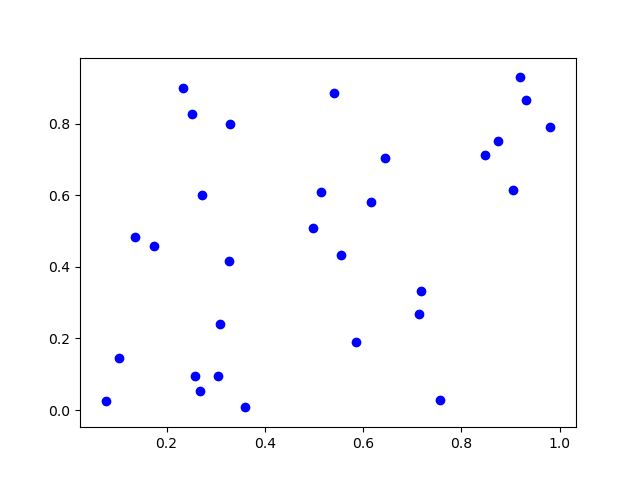
\includegraphics[width=0.5\textwidth]{../Figures/identifyModelGraph12CopyA.png}
\end{center}


The solution is \( \text{None of the above} \), which is option E.\begin{enumerate}[label=\Alph*.]
\item \( \text{Logarithmic model} \)

For this to be the correct option, we want a rapid change early, then an extremely slow change later.
\item \( \text{Linear model} \)

For this to be the correct option, we need to see a mostly straight line of points.
\item \( \text{Exponential model} \)

For this to be the correct option, we want an extremely slow change early, then a rapid change later.
\item \( \text{Non-linear Power model} \)

For this to be the correct option, we need to see a polynomial or rational shape.
\item \( \text{None of the above} \)

For this to be the correct option, we want to see no pattern in the points.
\end{enumerate}

\textbf{General Comment:} This question is testing if you can associate the models with their graphical representation. If you are having trouble, go back to the corresponding Core module to learn about the specific function you are having trouble recognizing.
}
\litem{
For the information provided below, construct a linear model that describes her total budget, $B$, as a function of the number of months, $x$ she is at UF.

\begin{center}
    \textit{ Aubrey is a college student going into her first year at UF. She will receive Bright Futures, which covers her tuition plus a \$800 educational expense each year. Before college, Aubrey saved up \$5000. She knows she will need to pay \$800 in rent a month, \$80 for food a week, and \$48 in other weekly expenses. }
\end{center}
The solution is \( B(x) = 5800 - 1312 x \), which is option D.\begin{enumerate}[label=\Alph*.]
\item \( B(x) = 4488 x \)

This treats the educational expense and savings as something you get every month rather than a 1-time payment.
\item \( B(x) = 4872 x \)

This treats the educational expense and savings as something you get every month rather than a 1-time payment AND treats weekly expenses as month expenses rather than multiplying each weekly expense by 4.
\item \( B(x) = 5800 - 928 x \)

This treats weekly expenses as month expenses rather than multiplying each weekly expense.
\item \( B(x) = 5800 - 1312 x \)

* This is the correct option.
\item \( \text{None of the above.} \)

You may have chosen this if you thought you were modeling total costs or income.
\end{enumerate}

\textbf{General Comment:} This is a Costs, Profit, Revenue question! The most common issues here are: (1) not converting the weekly costs to monthly costs, (2) treating the one-time values like savings and educational expense as happening per month, and (3) not checking that your model is for cost, profit [income], or revenue [budget].
}
\litem{
For the scenario below, use the model for the volume of a cylinder as $V = \pi r^2 h$.

\begin{center}
    \textit{ Pringles wants to add 27 \text{percent} more chips to their cylinder cans and minimize the design change of their cans. They've decided that the best way to minimize the design change is to increase the radius and height by the same percentage. What should this increase be? }
\end{center}
The solution is \( \text{About } 8 \text{ percent} \), which is option D.\begin{enumerate}[label=\Alph*.]
\item \( \text{About } 13 \text{ percent} \)

This corresponds to solving correctly but treating both radius and height as equal contributors to the volume.
\item \( \text{About } 14 \text{ percent} \)

This corresponds to treating both radius and height as equal contributors and not solving correctly.
\item \( \text{About } 3 \text{ percent} \)

This corresponds to not solving for the increase properly.
\item \( \text{About } 8 \text{ percent} \)

* This is the correct option.
\item \( \text{None of the above} \)

If you chose this, please contact the coordinator to discus how you solved the problem.
\end{enumerate}

\textbf{General Comment:} Remember that when plugging the increases of values in, you need to treat it as that percentage above 100. For example, a 5 percent increase means 105 percent.
}
\litem{
Solve the modeling problem below, if possible.

\begin{center}
    \textit{ In CHM2045L, Brittany created a 22 liter 21 percent solution of chemical $\chi$ using two different solution percentages of chemical $\chi$. When she went to write her lab report, she realized she forgot to write the amount of each solution she used! If she remembers she used 6 percent and 22 percent solutions, what was the amount she used of the 22 percent solution? }
\end{center}
The solution is \( 20.62 liters \), which is option B.\begin{enumerate}[label=\Alph*.]
\item \( 11.00 liters \)

This would be correct if Brittany used equal parts of each solution.
\item \( 20.62 liters \)

*This is the correct option.
\item \( 4.92 liters \)

This was a random value. If this was not a guess, contact the coordinator to talk about how you got this value.
\item \( 1.38 liters \)

This is the concentration of 6 percent solution.
\item \( \text{There is not enough information to solve the problem.} \)

You may have chose this if you thought you needed to know how much of the second solution was used in the problem. Remember that the total minus the first solution would give you the second amount used.
\end{enumerate}

\textbf{General Comment:} Build the model exactly as you did in Module 9M. Then, solve for the volume you are looking for.
}
\litem{
Solve the modeling problem below, if possible.

\begin{center}
    \textit{ A new virus is spreading throughout the world. There were initially 3 many cases reported, but the number of confirmed cases has tripled every 5 days. How long will it be until there are at least 1000 confirmed cases? }
\end{center}
The solution is \( \text{About } 27 \text{ days} \), which is option B.\begin{enumerate}[label=\Alph*.]
\item \( \text{About } 17 \text{ days} \)

You modeled the situation with $e$ as the base and did not apply the properties of log correctly.
\item \( \text{About } 27 \text{ days} \)

* This is the correct option.
\item \( \text{About } 16 \text{ days} \)

You modeled the situation correctly but did not apply the properties of log correctly.
\item \( \text{About } 30 \text{ days} \)

You modeled the situation with $e$ as the base, but solved correctly otherwise.
\item \( \text{There is not enough information to solve the problem.} \)

If you chose this option, please contact the coordinator to discuss why you think this is the case.
\end{enumerate}

\textbf{General Comment:} Set up the model the same as in Module 11M. Then, plug in 1000 and solve for $d$ in your model.
}
\litem{
Determine the appropriate model for the graph of points below.

\begin{center}
    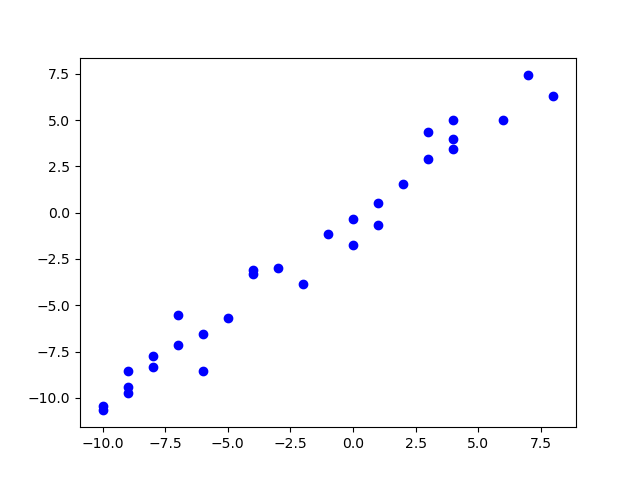
\includegraphics[width=0.5\textwidth]{../Figures/identifyModelGraph12B.png}
\end{center}


The solution is \( \text{Linear model} \), which is option A.\begin{enumerate}[label=\Alph*.]
\item \( \text{Linear model} \)

For this to be the correct option, we need to see a mostly straight line of points.
\item \( \text{Non-linear Power model} \)

For this to be the correct option, we need to see a polynomial or rational shape.
\item \( \text{Exponential model} \)

For this to be the correct option, we want an extremely slow change early, then a rapid change later.
\item \( \text{Logarithmic model} \)

For this to be the correct option, we want a rapid change early, then an extremely slow change later.
\item \( \text{None of the above} \)

For this to be the correct option, we want to see no pattern in the points.
\end{enumerate}

\textbf{General Comment:} This question is testing if you can associate the models with their graphical representation. If you are having trouble, go back to the corresponding Core module to learn about the specific function you are having trouble recognizing.
}
\litem{
For the scenario below, model the rate of vibration (cm/s) of the string in terms of the length of the string. Then determine the variation constant $k$ of the model (if possible). The constant should be in terms of cm and s.

\begin{center}
    \textit{ The rate of vibration of a string under constant tension varies based on the type of string and the length of the string. The rate of vibration of string $\omega$ decreases as the square length of the string increases. For example, when string $\omega$ is 2 mm long, the rate of vibration is 21 cm/s. }
\end{center}
The solution is \( k = 0.84 \), which is option C.\begin{enumerate}[label=\Alph*.]
\item \( k = 5.25 \)

This option uses the model $R = kl^{2}$ as if this is a direct variation AND does not convert from mm to cm so that the units match.
\item \( k = 84.00 \)

This option uses the correct model, $R = \frac{k}{l^{2}}$, but does not convert from mm to cm so that the units match.
\item \( k = 0.84 \)

* This is the correct option, which corresponds to the model $R = \frac{k}{l^{2}}$ AND converts from mm to cm.
\item \( k = 525.00 \)

This option uses the model $R = kl^{2}$ as if this is a direct variation.
\item \( \text{None of the above.} \)

Talk with the coordinator if you chose this option.
\end{enumerate}

\textbf{General Comment:} The most common mistake on this question is to not convert mm to cm! When modeling, you need to make sure all of the units for your variables are compatible.
}
\litem{
For the scenario below, use the model for the volume of a cylinder as $V = \pi r^2 h$.

\begin{center}
    \textit{ Pringles wants to add 36 \text{percent} more chips to their cylinder cans and minimize the design change of their cans. They've decided that the best way to minimize the design change is to increase the radius and height by the same percentage. What should this increase be? }
\end{center}
The solution is \( \text{About } 11 \text{ percent} \), which is option D.\begin{enumerate}[label=\Alph*.]
\item \( \text{About } 17 \text{ percent} \)

This corresponds to solving correctly but treating both radius and height as equal contributors to the volume.
\item \( \text{About } 3 \text{ percent} \)

This corresponds to not solving for the increase properly.
\item \( \text{About } 18 \text{ percent} \)

This corresponds to treating both radius and height as equal contributors and not solving correctly.
\item \( \text{About } 11 \text{ percent} \)

* This is the correct option.
\item \( \text{None of the above} \)

If you chose this, please contact the coordinator to discus how you solved the problem.
\end{enumerate}

\textbf{General Comment:} Remember that when plugging the increases of values in, you need to treat it as that percentage above 100. For example, a 5 percent increase means 105 percent.
}
\litem{
Solve the modeling problem below, if possible.

\begin{center}
    \textit{ In CHM2045L, Brittany created a 29 liter 22 percent solution of chemical $\chi$ using two different solution percentages of chemical $\chi$. When she went to write her lab report, she realized she forgot to write the amount of each solution she used! If she remembers she used 20 percent and 37 percent solutions, what was the amount she used of the 20 percent solution? }
\end{center}
The solution is \( 25.59 liters \), which is option C.\begin{enumerate}[label=\Alph*.]
\item \( 4.25 liters \)

This was a random value. If this was not a guess, contact the coordinator to talk about how you got this value.
\item \( 14.50 liters \)

This would be correct if Brittany used equal parts of each solution.
\item \( 25.59 liters \)

*This is the correct option.
\item \( 3.41 liters \)

This is the concentration of 37 percent solution.
\item \( \text{There is not enough information to solve the problem.} \)

You may have chose this if you thought you needed to know how much of the second solution was used in the problem. Remember that the total minus the first solution would give you the second amount used.
\end{enumerate}

\textbf{General Comment:} Build the model exactly as you did in Module 9M. Then, solve for the volume you are looking for.
}
\litem{
Solve the modeling problem below, if possible.

\begin{center}
    \textit{ A new virus is spreading throughout the world. There were initially 4 many cases reported, but the number of confirmed cases has doubled every 4 days. How long will it be until there are at least 1000 confirmed cases? }
\end{center}
The solution is \( \text{About } 32 \text{ days} \), which is option D.\begin{enumerate}[label=\Alph*.]
\item \( \text{About } 12 \text{ days} \)

You modeled the situation with $e$ as the base and did not apply the properties of log correctly.
\item \( \text{About } 14 \text{ days} \)

You modeled the situation correctly but did not apply the properties of log correctly.
\item \( \text{About } 23 \text{ days} \)

You modeled the situation with $e$ as the base, but solved correctly otherwise.
\item \( \text{About } 32 \text{ days} \)

* This is the correct option.
\item \( \text{There is not enough information to solve the problem.} \)

If you chose this option, please contact the coordinator to discuss why you think this is the case.
\end{enumerate}

\textbf{General Comment:} Set up the model the same as in Module 11M. Then, plug in 1000 and solve for $d$ in your model.
}
\litem{
Determine the appropriate model for the graph of points below.

\begin{center}
    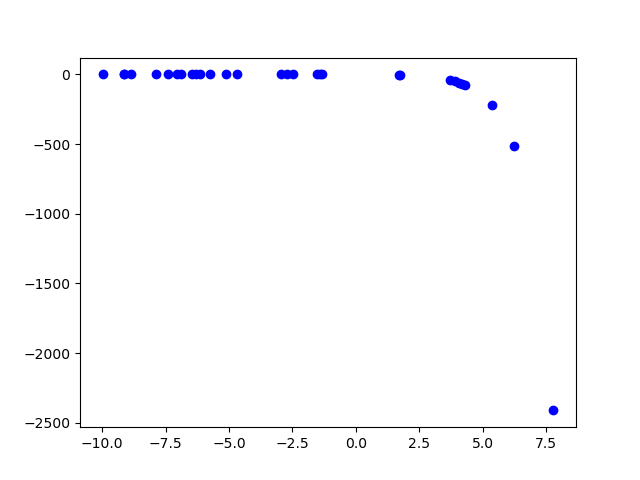
\includegraphics[width=0.5\textwidth]{../Figures/identifyModelGraph12CopyB.png}
\end{center}


The solution is \( \text{Exponential model} \), which is option B.\begin{enumerate}[label=\Alph*.]
\item \( \text{Non-linear Power model} \)

For this to be the correct option, we need to see a polynomial or rational shape.
\item \( \text{Exponential model} \)

For this to be the correct option, we want an extremely slow change early, then a rapid change later.
\item \( \text{Linear model} \)

For this to be the correct option, we need to see a mostly straight line of points.
\item \( \text{Logarithmic model} \)

For this to be the correct option, we want a rapid change early, then an extremely slow change later.
\item \( \text{None of the above} \)

For this to be the correct option, we want to see no pattern in the points.
\end{enumerate}

\textbf{General Comment:} This question is testing if you can associate the models with their graphical representation. If you are having trouble, go back to the corresponding Core module to learn about the specific function you are having trouble recognizing.
}
\litem{
For the information below, construct a linear model that describes the total time $T$ spent on the path in terms of the distance of a particular part of the path \textit{if we know that all parts of the path are equal length}.

\begin{center}
    \textit{ A bicyclist is training for a race on a hilly path. Their bike keeps track of their speed at any time, but not the distance traveled. Their speed traveling up a hill is 5 mph, 10 mph when traveling down a hill, and 8 mph when traveling along a flat portion. }
\end{center}
The solution is \( 0.425 D \), which is option B.\begin{enumerate}[label=\Alph*.]
\item \( 400.000 D \)

The coefficient here is calculated by multiplying the distances together rather than adding.
\item \( 0.425 D \)

* This is the correct option.
\item \( 23.000 D \)

The coefficient here is calculated as if you were trying to model the distance on the total path.
\item \( \text{The model can be found with the information provided, but isn't options 1-3.} \)

Since we know all parts of the path are equal length, we can treat all distance variables as the same variable, $D$.
\item \( \text{The model cannot be found with the information provided.} \)

If you chose this option, please contact the coordinator to discuss why you think we cannot model the situation.
\end{enumerate}

\textbf{General Comment:} Be sure you pay attention to the variable we are writing the model in terms of. To create the model with a single variable, we have to know that variable is the same throughout each path!
}
\litem{
For the scenario below, use the model for the volume of a cylinder as $V = \pi r^2 h$.

\begin{center}
    \textit{ Pringles wants to add 38 \text{percent} more chips to their cylinder cans and minimize the design change of their cans. They've decided that the best way to minimize the design change is to increase the radius and height by the same percentage. What should this increase be? }
\end{center}
The solution is \( \text{About } 11 \text{ percent} \), which is option A.\begin{enumerate}[label=\Alph*.]
\item \( \text{About } 11 \text{ percent} \)

* This is the correct option.
\item \( \text{About } 3 \text{ percent} \)

This corresponds to not solving for the increase properly.
\item \( \text{About } 19 \text{ percent} \)

This corresponds to treating both radius and height as equal contributors and not solving correctly.
\item \( \text{About } 17 \text{ percent} \)

This corresponds to solving correctly but treating both radius and height as equal contributors to the volume.
\item \( \text{None of the above} \)

If you chose this, please contact the coordinator to discus how you solved the problem.
\end{enumerate}

\textbf{General Comment:} Remember that when plugging the increases of values in, you need to treat it as that percentage above 100. For example, a 5 percent increase means 105 percent.
}
\litem{
Solve the modeling problem below, if possible.

\begin{center}
    \textit{ In CHM2045L, Brittany created a 23 liter 29 percent solution of chemical $\chi$ using two different solution percentages of chemical $\chi$. When she went to write her lab report, she realized she forgot to write the amount of each solution she used! If she remembers she used 15 percent and 37 percent solutions, what was the amount she used of the 15 percent solution? }
\end{center}
The solution is \( 8.36 liters \), which is option D.\begin{enumerate}[label=\Alph*.]
\item \( 14.64 liters \)

This is the concentration of 37 percent solution.
\item \( 10.14 liters \)

This was a random value. If this was not a guess, contact the coordinator to talk about how you got this value.
\item \( 11.50 liters \)

This would be correct if Brittany used equal parts of each solution.
\item \( 8.36 liters \)

*This is the correct option.
\item \( \text{There is not enough information to solve the problem.} \)

You may have chose this if you thought you needed to know how much of the second solution was used in the problem. Remember that the total minus the first solution would give you the second amount used.
\end{enumerate}

\textbf{General Comment:} Build the model exactly as you did in Module 9M. Then, solve for the volume you are looking for.
}
\litem{
Solve the modeling problem below, if possible.

\begin{center}
    \textit{ A new virus is spreading throughout the world. There were initially 4 many cases reported, but the number of confirmed cases has doubled every 1 days. How long will it be until there are at least 100000 confirmed cases? }
\end{center}
The solution is \( \text{About } 15 \text{ days} \), which is option A.\begin{enumerate}[label=\Alph*.]
\item \( \text{About } 15 \text{ days} \)

* This is the correct option.
\item \( \text{About } 5 \text{ days} \)

You modeled the situation with $e$ as the base and did not apply the properties of log correctly.
\item \( \text{About } 11 \text{ days} \)

You modeled the situation with $e$ as the base, but solved correctly otherwise.
\item \( \text{About } 6 \text{ days} \)

You modeled the situation correctly but did not apply the properties of log correctly.
\item \( \text{There is not enough information to solve the problem.} \)

If you chose this option, please contact the coordinator to discuss why you think this is the case.
\end{enumerate}

\textbf{General Comment:} Set up the model the same as in Module 11M. Then, plug in 100000 and solve for $d$ in your model.
}
\litem{
Determine the appropriate model for the graph of points below.

\begin{center}
    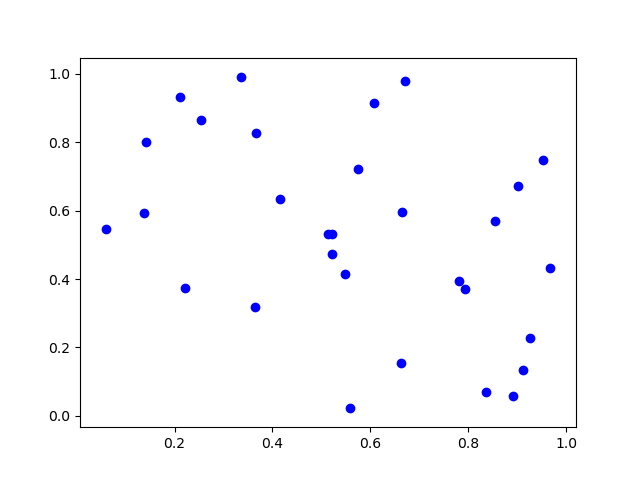
\includegraphics[width=0.5\textwidth]{../Figures/identifyModelGraph12C.png}
\end{center}


The solution is \( \text{None of the above} \), which is option E.\begin{enumerate}[label=\Alph*.]
\item \( \text{Non-linear Power model} \)

For this to be the correct option, we need to see a polynomial or rational shape.
\item \( \text{Linear model} \)

For this to be the correct option, we need to see a mostly straight line of points.
\item \( \text{Logarithmic model} \)

For this to be the correct option, we want a rapid change early, then an extremely slow change later.
\item \( \text{Exponential model} \)

For this to be the correct option, we want an extremely slow change early, then a rapid change later.
\item \( \text{None of the above} \)

For this to be the correct option, we want to see no pattern in the points.
\end{enumerate}

\textbf{General Comment:} This question is testing if you can associate the models with their graphical representation. If you are having trouble, go back to the corresponding Core module to learn about the specific function you are having trouble recognizing.
}
\litem{
The temperature of an object, $T$, in a different surrounding temperature $T_s$ will behave according to the formula $T(t) = Ae^{kt} + T_s$, where $t$ is minutes, $A$ is a constant, and k is a constant. Use this formula and the situation below to construct a model that describes the uranium's temperature, $T$, based on the amount of time t (in minutes) that have passed. Choose the correct constant $k$ from the options below.

\begin{center}
    \textit{ Uranium is taken out of the reactor with a temperature of $180^{\circ}$ C and is placed into a $17^{\circ}$ C bath to cool. After 30 minutes, the uranium has cooled to $116^{\circ}$ C. }
\end{center}
The solution is \( k = -0.01662 \), which is option D.\begin{enumerate}[label=\Alph*.]
\item \( k = -0.02473 \)

This uses $A$ as the initial temperature and solves for $k$ incorrectly.
\item \( k = -0.01993 \)

This uses $A$ as the initial temperature and solves for $k$ correctly.
\item \( k = -0.02514 \)

This uses $A$ correctly but solves for $k$ incorrectly.
\item \( k = -0.01662 \)

* This is the correct option.
\item \( \text{None of the above} \)

If you chose this, please contact the coordinator to discuss why you believe none of the other answers are correct.
\end{enumerate}

\textbf{General Comment:} The initial temperature is when $t = 0$. Unlike power models, that means $A$ is not the initial temperature!
}
\litem{
For the scenario below, use the model for the volume of a cylinder as $V = \pi r^2 h$.

\begin{center}
    \textit{ Pringles wants to add 27 \text{percent} more chips to their cylinder cans and minimize the design change of their cans. They've decided that the best way to minimize the design change is to increase the radius and height by the same percentage. What should this increase be? }
\end{center}
The solution is \( \text{About } 8 \text{ percent} \), which is option B.\begin{enumerate}[label=\Alph*.]
\item \( \text{About } 13 \text{ percent} \)

This corresponds to solving correctly but treating both radius and height as equal contributors to the volume.
\item \( \text{About } 8 \text{ percent} \)

* This is the correct option.
\item \( \text{About } 9 \text{ percent} \)

This corresponds to not solving for the increase properly.
\item \( \text{About } 14 \text{ percent} \)

This corresponds to treating both radius and height as equal contributors and not solving correctly.
\item \( \text{None of the above} \)

If you chose this, please contact the coordinator to discus how you solved the problem.
\end{enumerate}

\textbf{General Comment:} Remember that when plugging the increases of values in, you need to treat it as that percentage above 100. For example, a 5 percent increase means 105 percent.
}
\litem{
Solve the modeling problem below, if possible.

\begin{center}
    \textit{ In CHM2045L, Brittany created a 15 liter 15 percent solution of chemical $\chi$ using two different solution percentages of chemical $\chi$. When she went to write her lab report, she realized she forgot to write the amount of each solution she used! If she remembers she used 7 percent and 37 percent solutions, what was the amount she used of the 37 percent solution? }
\end{center}
The solution is \( 4.00 liters \), which is option D.\begin{enumerate}[label=\Alph*.]
\item \( 7.50 liters \)

This would be correct if Brittany used equal parts of each solution.
\item \( 11.00 liters \)

This is the concentration of 7 percent solution.
\item \( 5.62 liters \)

This was a random value. If this was not a guess, contact the coordinator to talk about how you got this value.
\item \( 4.00 liters \)

*This is the correct option.
\item \( \text{There is not enough information to solve the problem.} \)

You may have chose this if you thought you needed to know how much of the second solution was used in the problem. Remember that the total minus the first solution would give you the second amount used.
\end{enumerate}

\textbf{General Comment:} Build the model exactly as you did in Module 9M. Then, solve for the volume you are looking for.
}
\litem{
Solve the modeling problem below, if possible.

\begin{center}
    \textit{ A new virus is spreading throughout the world. There were initially 5 many cases reported, but the number of confirmed cases has doubled every 2 days. How long will it be until there are at least 1000000 confirmed cases? }
\end{center}
The solution is \( \text{About } 36 \text{ days} \), which is option A.\begin{enumerate}[label=\Alph*.]
\item \( \text{About } 36 \text{ days} \)

* This is the correct option.
\item \( \text{About } 12 \text{ days} \)

You modeled the situation correctly but did not apply the properties of log correctly.
\item \( \text{About } 11 \text{ days} \)

You modeled the situation with $e$ as the base and did not apply the properties of log correctly.
\item \( \text{About } 25 \text{ days} \)

You modeled the situation with $e$ as the base, but solved correctly otherwise.
\item \( \text{There is not enough information to solve the problem.} \)

If you chose this option, please contact the coordinator to discuss why you think this is the case.
\end{enumerate}

\textbf{General Comment:} Set up the model the same as in Module 11M. Then, plug in 1000000 and solve for $d$ in your model.
}
\litem{
Determine the appropriate model for the graph of points below.

\begin{center}
    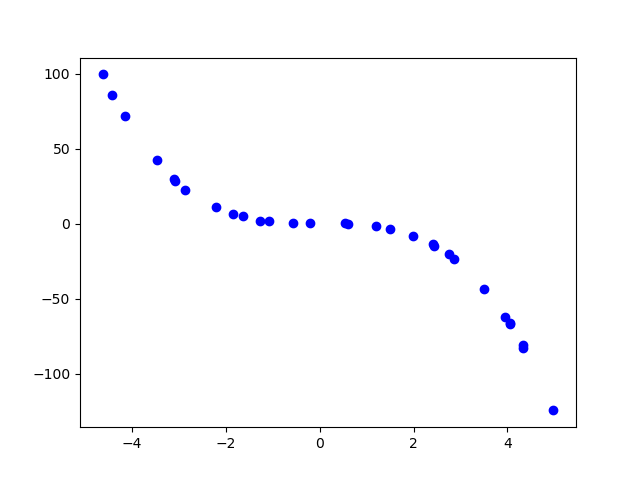
\includegraphics[width=0.5\textwidth]{../Figures/identifyModelGraph12CopyC.png}
\end{center}


The solution is \( \text{Non-linear Power model} \), which is option B.\begin{enumerate}[label=\Alph*.]
\item \( \text{Exponential model} \)

For this to be the correct option, we want an extremely slow change early, then a rapid change later.
\item \( \text{Non-linear Power model} \)

For this to be the correct option, we need to see a polynomial or rational shape.
\item \( \text{Logarithmic model} \)

For this to be the correct option, we want a rapid change early, then an extremely slow change later.
\item \( \text{Linear model} \)

For this to be the correct option, we need to see a mostly straight line of points.
\item \( \text{None of the above} \)

For this to be the correct option, we want to see no pattern in the points.
\end{enumerate}

\textbf{General Comment:} This question is testing if you can associate the models with their graphical representation. If you are having trouble, go back to the corresponding Core module to learn about the specific function you are having trouble recognizing.
}
\litem{
For the scenario below, use the model for the volume of a cylinder as $V = \pi r^2 h$ to find the coefficient for the model of the new volume $V_{\text{new}} = k r^2 h$.

\begin{center}
    \textit{ Pepsi wants to increase the volume of soda in their cans. They've decided to decrease the radius by 15 percent and decrease the height by 14 percent. They want to model the new volume based on the radius and height of the original cans. }
\end{center}
The solution is \( k = 1.95203 \), which is option C.\begin{enumerate}[label=\Alph*.]
\item \( k = 0.62135 \)

This corresponds to the model: $V = (0.85 r)^2 (0.86 h)$.
\item \( k = 0.00315 \)

This corresponds to the model: $V = (0.15 r)^2 (0.14 h)$.
\item \( k = 1.95203 \)

* This is the correct option and corresponds to the model: $V = \pi (0.85 r)^2 (0.86 h)$.
\item \( k = 0.00990 \)

This corresponds to the model: $V = \pi (0.15 r)^2 (0.14 h)$.
\item \( \text{None of the above.} \)

If you chose this, please talk with the coordinator to discuss why you believe none of the options are correct.
\end{enumerate}

\textbf{General Comment:} When calculating the new dimensions, you need to add/subtract from 100\%. For example, a 10\% increase in height would result in 110\% of the original height: $1.1h_{old} = h_{new}$.
}
\end{enumerate}

\end{document}